
\documentclass{article}
\usepackage{pgfplots}
\usepackage{pgfplotstable}
\usepackage{tikz}
\pgfplotsset{compat=1.8}
\begin{document}
    \begin{figure*}[t]
        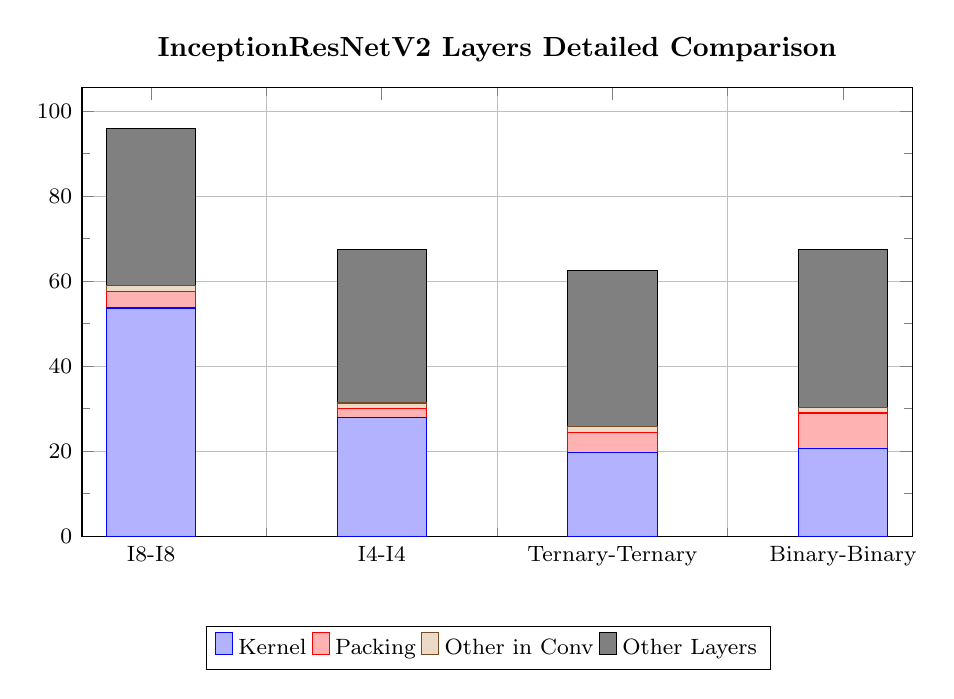
\begin{tikzpicture}
            \begin{axis}[
                ybar stacked,
                ymin=0.0,
                width=\linewidth,
                height=\axisdefaultheight,
                tick label style={font=\footnotesize},
                legend style={font=\tiny},
                label style={font=\footnotesize},
                symbolic x coords={I8-I8, I4-I4, Ternary-Ternary, Binary-Binary},
                xtick=data,
                % ytick={0.60,0.80,1.0,1.2,1.4,1.6,1.8,2.0,2.2,2.4,2.6,2.8,3.0},
                align={center},
                bar width=7.5ex,
                legend columns=7,
                legend style={at={(0.49,-0.2)},anchor=north,font=\footnotesize},
                title=\textbf{InceptionResNetV2 Layers Detailed Comparison},
                ymajorgrids,
                xminorgrids = true,
                minor tick num=1
                ]
                \addplot coordinates { (I8-I8,53.70) (I4-I4,27.86) (Ternary-Ternary,19.74) (Binary-Binary,20.58) };
                \addplot coordinates { (I8-I8,3.88) (I4-I4,2.12) (Ternary-Ternary,4.62) (Binary-Binary,8.40) };
                \addplot coordinates { (I8-I8,1.42) (I4-I4,1.37) (Ternary-Ternary,1.38) (Binary-Binary,1.37) };
                \addplot coordinates { (I8-I8,36.91) (I4-I4,36.12) (Ternary-Ternary,36.77) (Binary-Binary,37.17) };
                \legend{
                    Kernel,
                    Packing,
                    Other in Conv,
                    Other Layers,
                };
            \end{axis}
        \end{tikzpicture}
    \end{figure*}
\end{document}
